\documentclass[14pt,t]{beamer}
\usepackage{pslatex,adjustbox}
\usepackage{caption}
\usepackage{subcaption}
\captionsetup{compatibility=false}
\usetheme[unit=ics]{Frederiksberg}
\useinnertheme{MLHacks}

\AtBeginSection[]
{
	\begin{frame}{Agenda}
		\tableofcontents[currentsection]
		\ghostframe
	\end{frame}
}

\title{A study of higher order \\ image descriptors}
\subtitle{Thesis defence}
\author{Benjamin Braithwaite \\\and Malte Nissen}
\institute{Department of Computer Science}
\date[]{\today}
%
\begin{document}
%
\frame[plain]{\titlepage}
%
\begin{frame}{Agenda}
	\tableofcontents
\end{frame}
%
\section{Introduction to image descriptors}
%
\begin{frame}{Image transformations}
\begin{figure}
\centering
	\begin{subfigure}[t]{0.4\textwidth}
		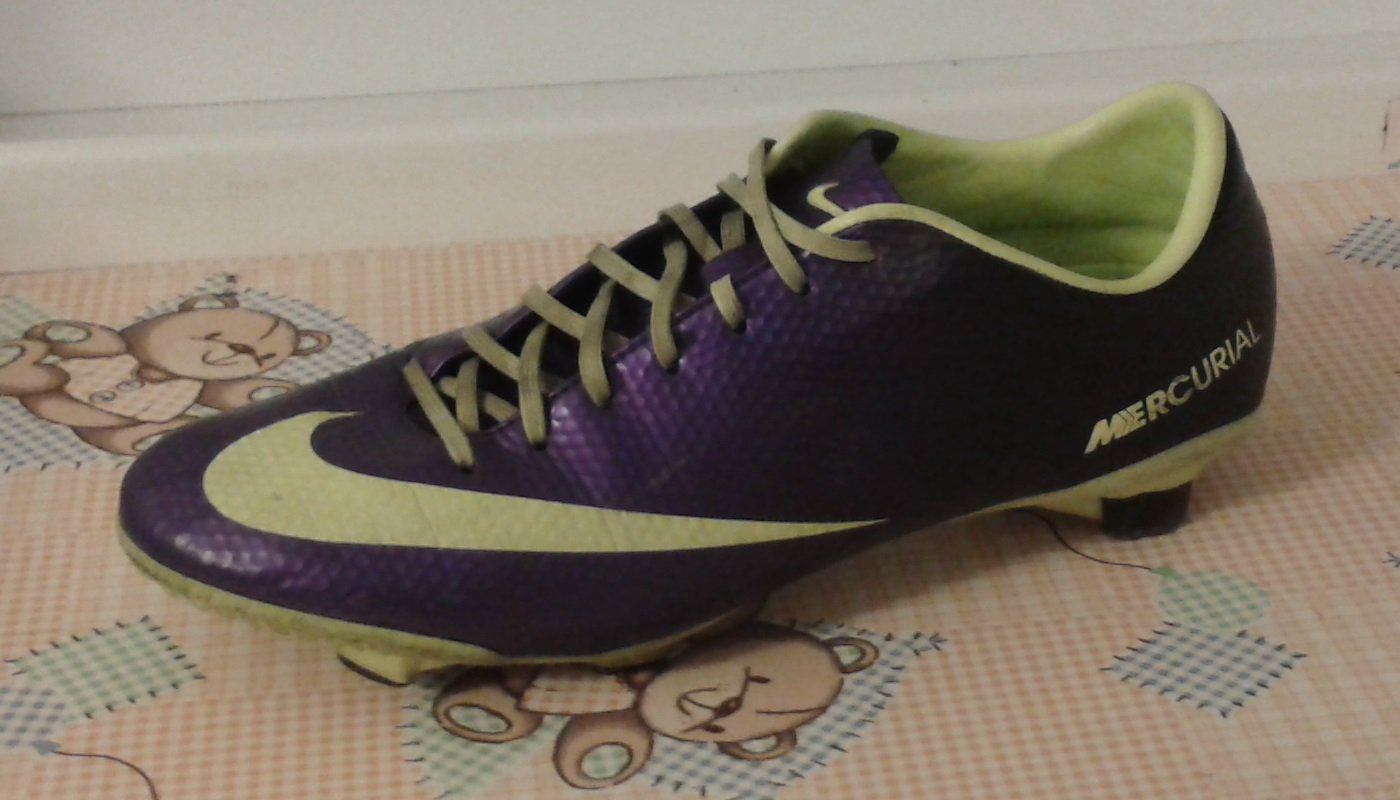
\includegraphics[width=\textwidth]{img/shoeOriginal.jpg}
	\end{subfigure}\\
	\vspace{0.75mm}
	\begin{subfigure}[t]{0.4\textwidth}
		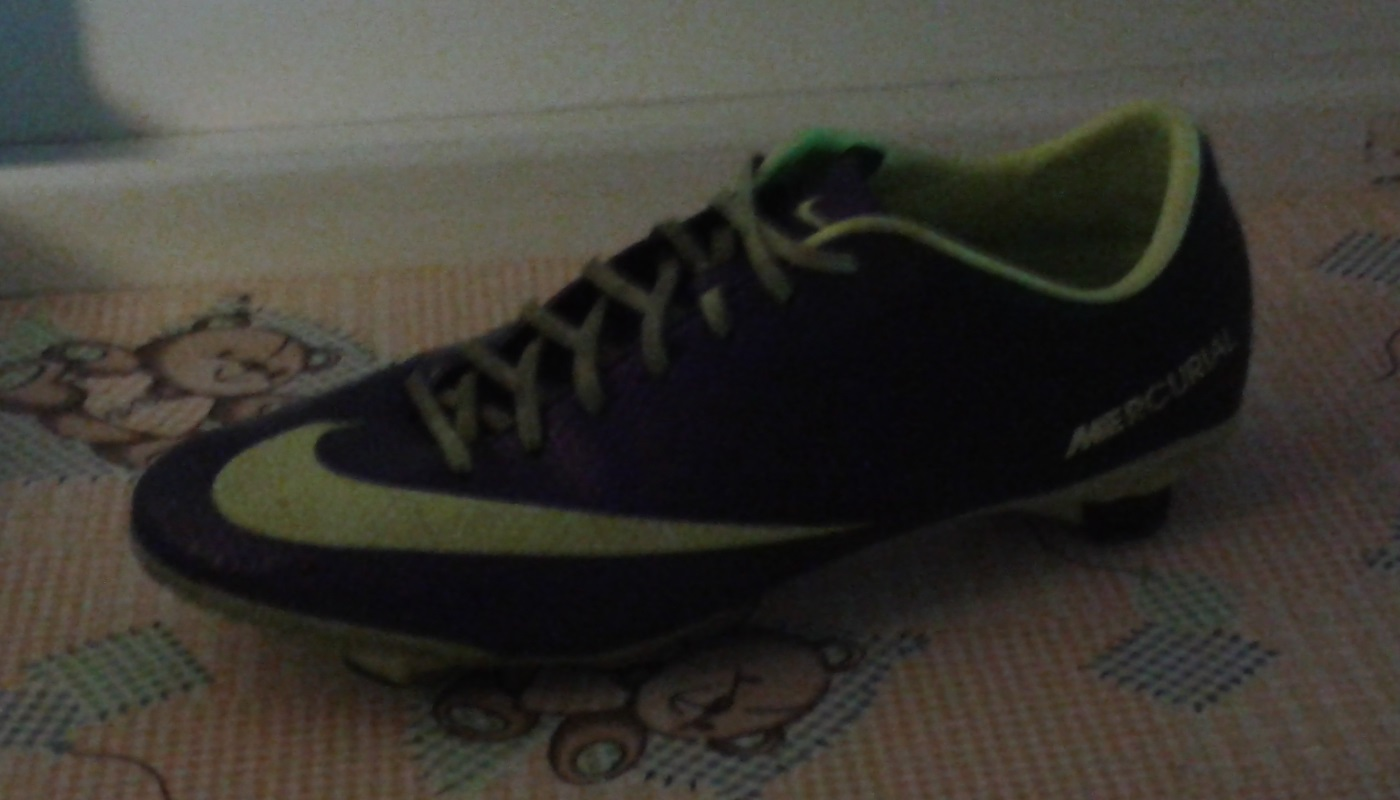
\includegraphics[width=\textwidth]{img/shoeDark.jpg}
	\end{subfigure}
	\begin{subfigure}[t]{0.4\textwidth}
		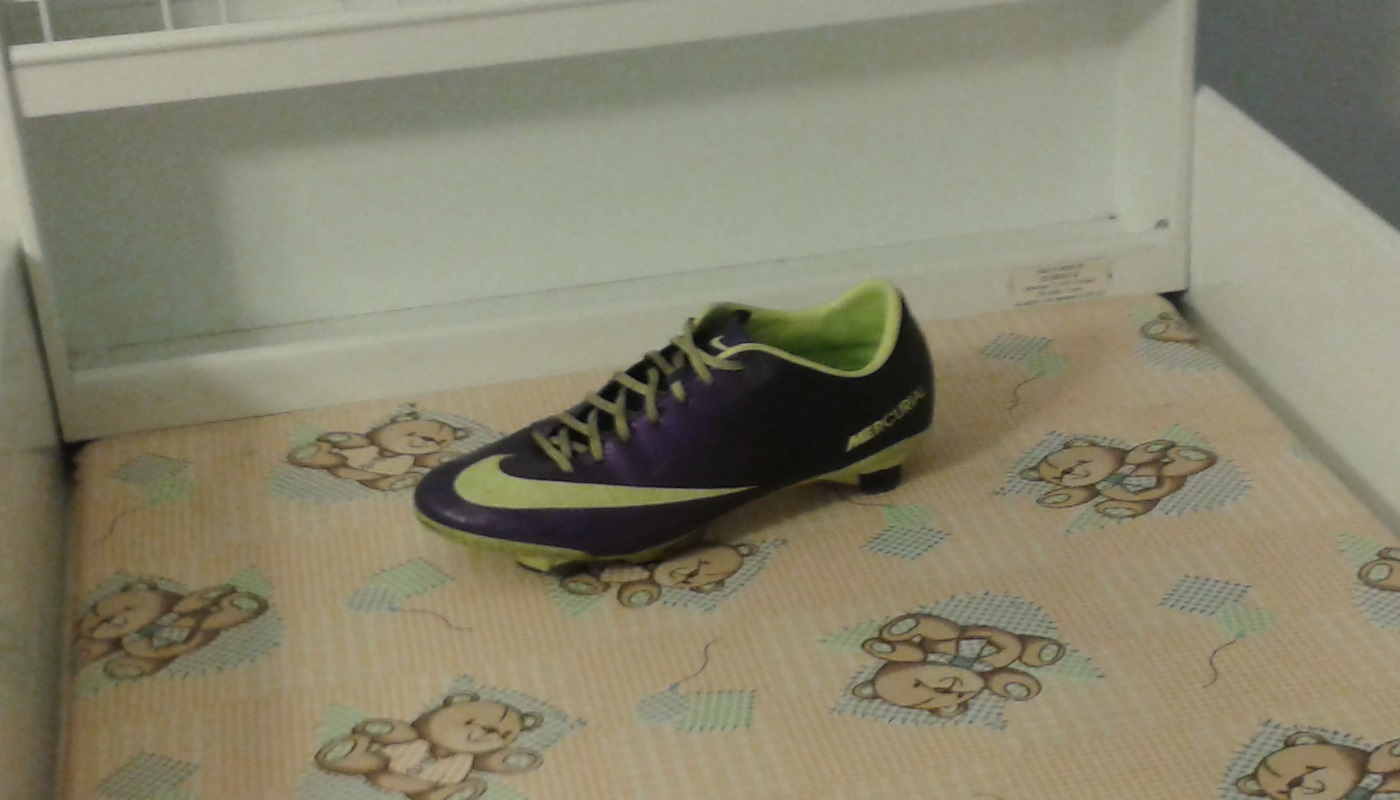
\includegraphics[width=\textwidth]{img/shoeScale.jpg}
	\end{subfigure}\\
	\vspace{0.75mm}
	\begin{subfigure}[t]{0.4\textwidth}
		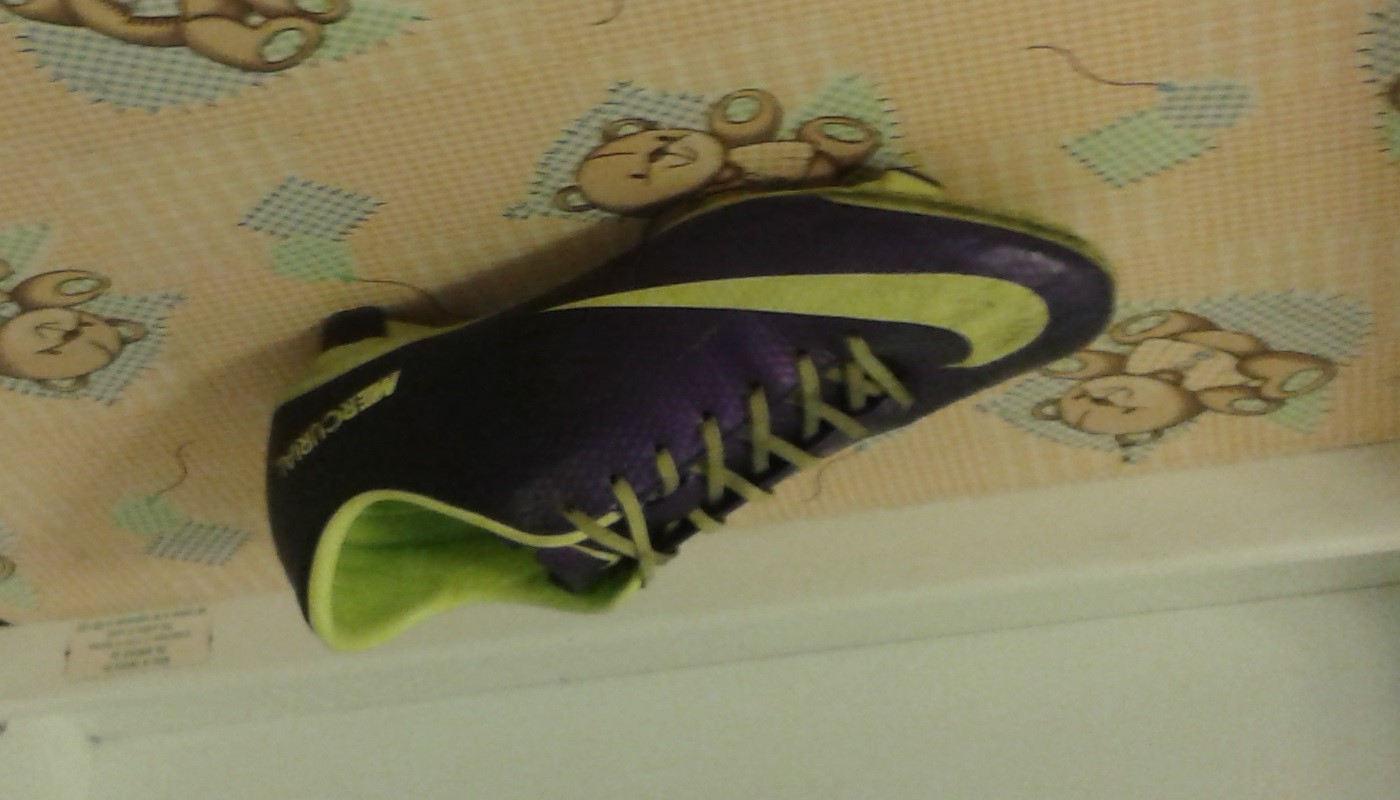
\includegraphics[width=\textwidth]{img/shoeRotation.jpg}
	\end{subfigure}
	\begin{subfigure}[t]{0.4\textwidth}
		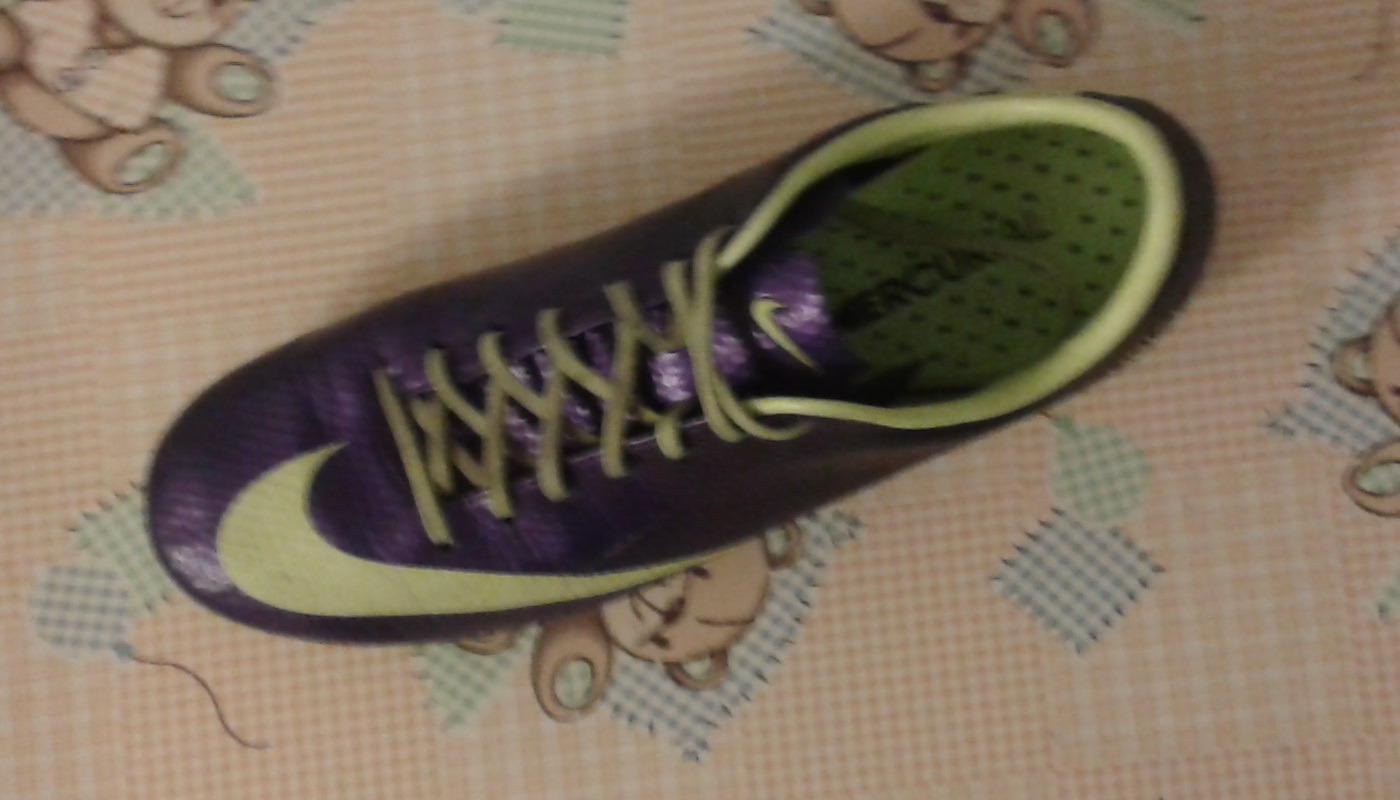
\includegraphics[width=\textwidth]{img/shoeAbove.jpg}
	\end{subfigure}
\end{figure}
\end{frame}
%
\begin{frame}{Applications}
\begin{figure}
\centering
	\begin{subfigure}[t]{0.49\textwidth}
		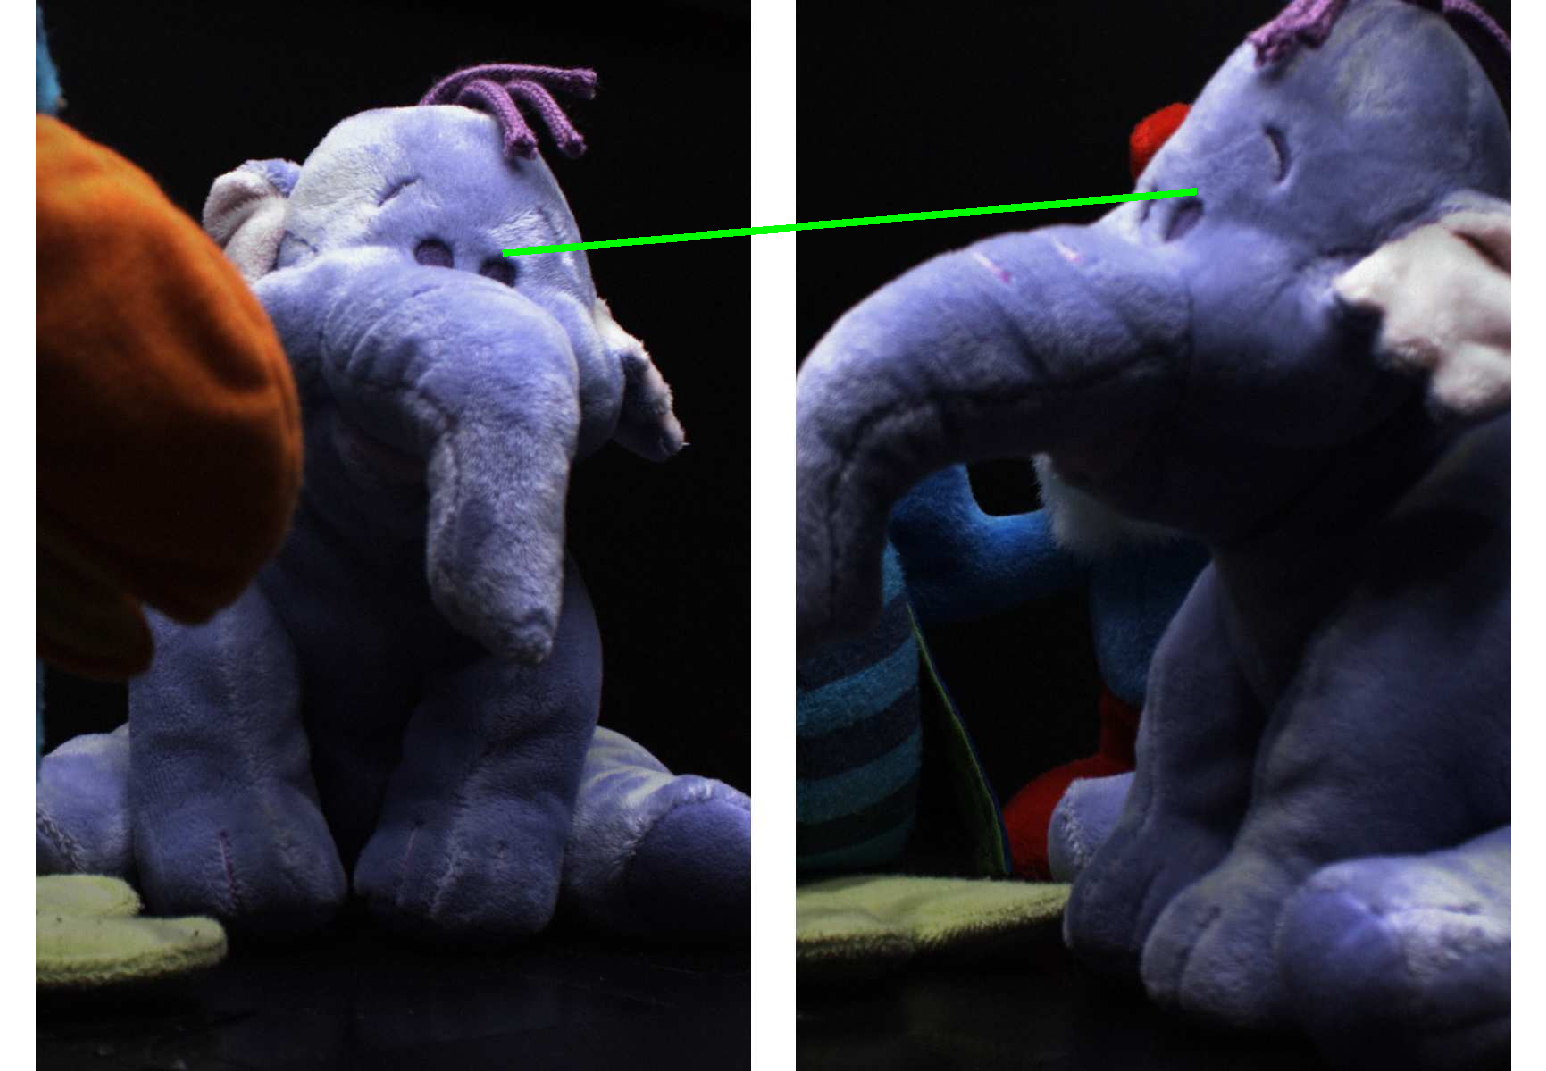
\includegraphics[width=\textwidth]{../report/img/introductionIC.pdf}
		\caption{Image correspondence}
	\end{subfigure}
	\begin{subfigure}[t]{0.49\textwidth}
		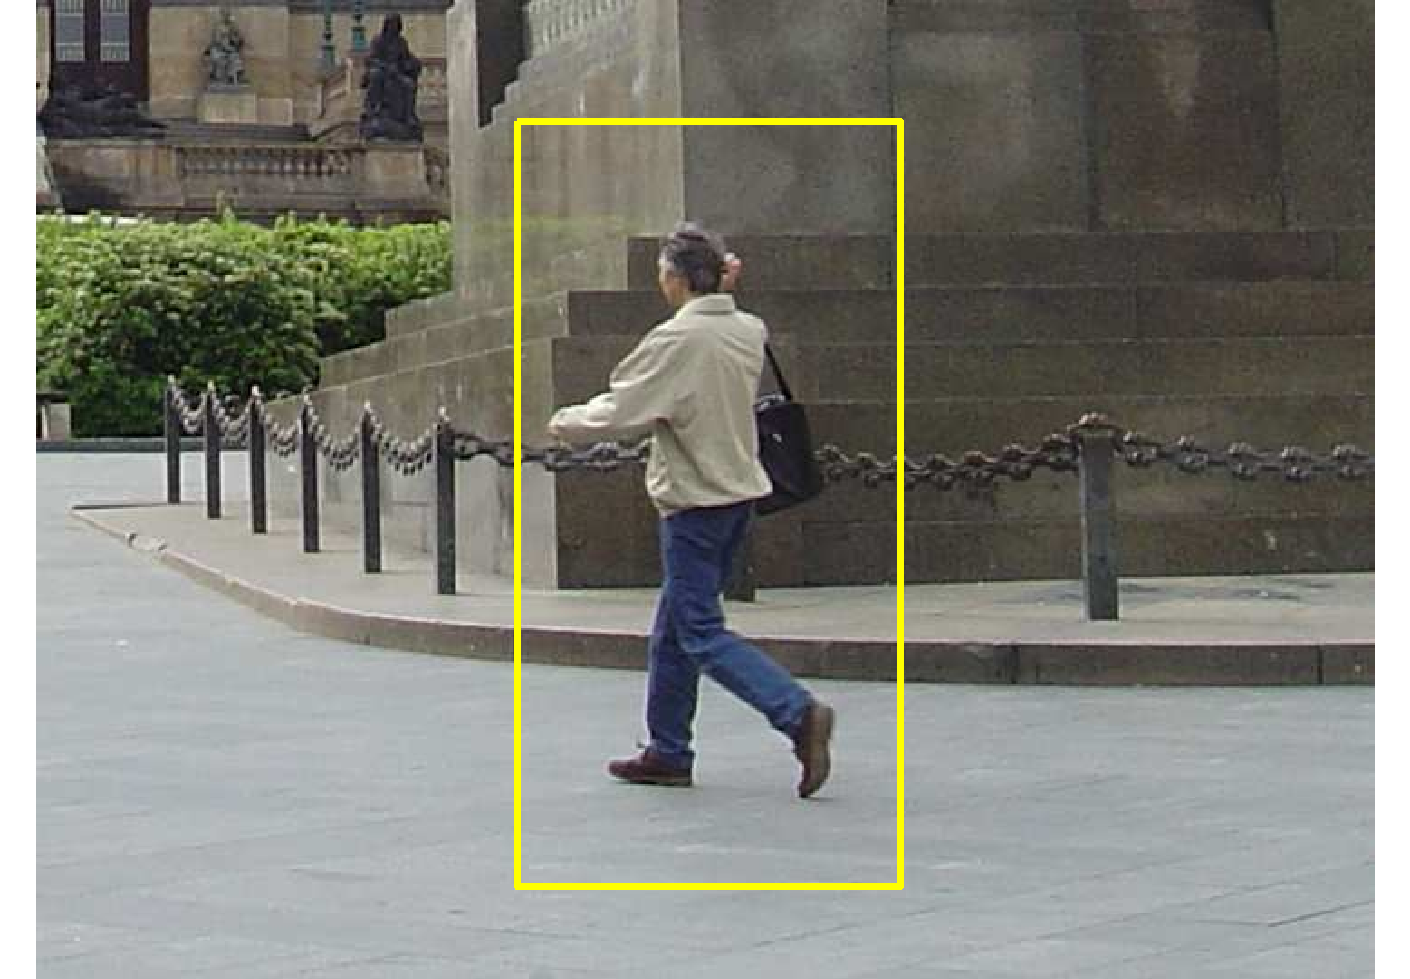
\includegraphics[width=\textwidth]{../report/img/introductionOD.pdf}
		\caption{Pedestrian detection}
	\end{subfigure}
\end{figure}
\end{frame}
%
\section{Image correspondence}
%

%
\section{Pedestrian detection}
%
%\begin{frame}{Radon transform}
%\begin{figure}
%\centering
%\adjincludegraphics[scale=.4,trim={80 80 80 80}]{radon_example.pdf}
%\label{fig:radon_example}
%\end{figure}
%\end{frame}
%
\end{document}